\graphicspath{{./assets/}}
\setcounter{mtc}{7}
\chapter{5th Sprint : Initial PaaS setup}
\fancyhead[R]{\small\textbf{Chapter VII. 5th Sprint: Initial PaaS setup  }}

\minitoc
\newpage
\section*{Introduction}
In this chapter, we will explore the process of setting up the Kubernetes-based PaaS. Our PaaS will include Traefik, a powerful ingress controller that provides load balancing and routing capabilities, MetalLB, a load balancer that simplifies network configuration, and Ceph, a distributed storage system that provides scalability and high availability.

We will use Ansible to automate the deployment of our PaaS environment.

\section{Sprint backlog :}

\begin{longtable}[H]{|m{1.5cm}|m{3cm}|m{1.5cm}|m{9cm}|}
\hline
{\textbf{Epic ID}} & {\textbf{Epic}} & {\textbf{Story ID}} & {\textbf{Story}}\\
\hline
1  & PaaS setup: Setting the service groups for networking and storage	 &  1.1	 &  Setting up the ingress controller (traefik).\\
\cline{3-4}
& & 1.2 & Setting up the network level load balancer (metalLB). \\
\cline{3-4}
& & 1.3	& Setting up the load balancer. \\
\cline{3-4}
\hline
\caption{5th Sprint Backlog}
\end{longtable}


\section{UML design: package diagram for the initial PaaS setup}

Here, the PaaS is the main package and contains all the other packages.

Within the PaaS package, there are three sub-packages: the Kubernetes control plane, Traefik/MetalLB, and Ceph. The control plane package contains all of the components necessary for running Kubernetes (e.g., etcd, kube-proxy, etc.), while the Traefik/MetalLB package contains the Traefik and MetalLB components used for ingress and load balancing, respectively.

Finally, the Ceph package contains all of the necessary components for running distributed storage using Ceph.

\begin{figure}[H]\centering
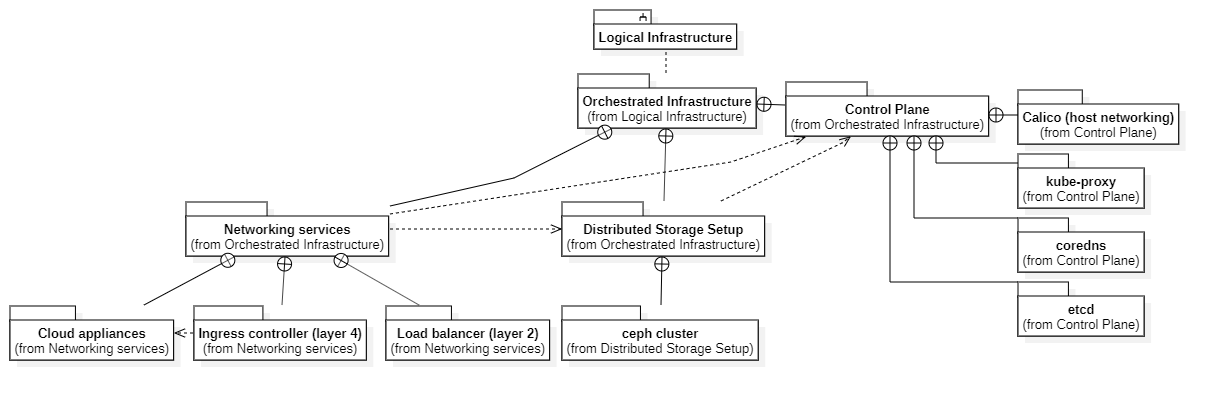
\includegraphics[width=1.0\textwidth,angle=00]{assets/f21.png}
\caption{ Package diagram for the initial PaaS setup }
\label{fig:package diagram for the initial PaaS setup}
\end{figure}

\section{Networking services}

\subsection{Overview on the networking services}

As illustrated in the following figure, Traefik, Cert-manager, and MetalLB work together to provide a secure and scalable way to route traffic inside Kubernetes using Services and IngressRoutes.

\begin{figure}[H]\centering
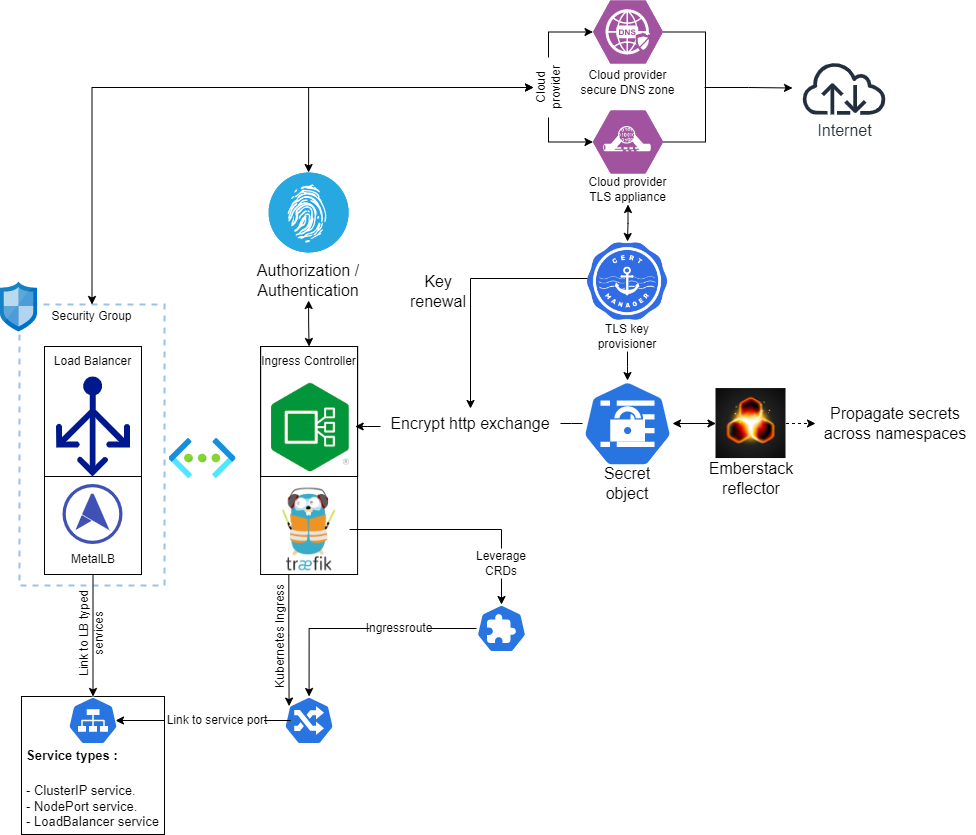
\includegraphics[width=1.0\textwidth,angle=00]{assets/f22.png}
\caption{ Networking services}
\label{fig:Networking services}
\end{figure}

Taking into consideration the following setup :
\begin{enumerate}
\item Application workloads are exposed through services of different types:
    \begin{itemize}[label={--}]
        \item ClusterIP: access from within the cluster access.
        \item LoadBalancer: access from outside the cluster using the external ip allocated through the loadbalancer.
        \item NodePort: access from outside the cluster using the ip of the node on which the application container is running.
    \end{itemize}

\item Cert-manager is configured as a cluster issuer and uses a "DNS challenge" to provision TLS certificates specific to every subdomain or domain.

\item Cert-manager listens to every declared "certificate" resource in order to process it and generate a valid "TLS certificate" that is then stored in a secret.

\item Cert-manager is configured to renew the generated certificates periodically.

\item Emberstack reflector is used to propagate secrets and configmaps across namespaces.

The flow is as follows:

\item Traffic enters from the Internet and is directed either to MetalLB for network level load balancing, or to the Traefik ingress controller for application level load balancing.

\item Traefik Proxy receives the traffic and routes it to the appropriate Kubernetes Service that is linked to a previously configured ingressroute, based on the domain name in the request.

\item The Service forwards the traffic to the appropriate Kubernetes Pod.

\item IngressRoutes are defined for workload, and Traefik uses these IngressRoutes to direct traffic to the appropriate Service.

\item Traefik is configured to use the TLS certificates generated by Cert-manager to terminate SSL/TLS traffic.

\item Traffic is routed to the correct Kubernetes Pods based on the domain name in the request.

\item The Kubernetes Pods process the requests and respond to the Traefik Proxy.

\item Traefik handles TLS termination using the secrets previously generated a
\end{enumerate}

\subsection{Secret provisioning and propagation:}

\subsubsection{TLS secret provisioning:}

In order to provide secure HTTPS communications between clients and the deployed workloads, valid TLS certificates need to be provisioned from our provider tls appliances. Our tool of choice is cert-manager.

Cert-manager provides us with a powerful and flexible way to manage TLS certificates in Kubernetes, enabling automatic provisioning and renewal of certificates from various certificate authorities, namely: "OVH Cloud Provider" and "Cloudflare".

By automating certificate management, cert-manager helps improve the security and reliability of our Kubernetes services, while reducing the operational burden of manual certificate provisioning and management.

Leveraging the capabilities of cert-manager is summarized by the following steps:

\begin{enumerate}
    \item  Having setup the stock cert-manager deployment, we first create the "ClusterIssuer" Kubernetes resource. Here we showcase a sample manifest:
        \begin{listing}[H]
        \inputminted{Yaml}{codeListing/cert_manager_cluster_issuer.yml}
        \caption{Cert manager cluster issuer}
        \label{lst:the-code}
        \end{listing}
    The cluster issuer manifest contains the credentials cert-manager uses to authenticate with our domain registrar (OVH). It needs these credentials to perform a DNS-01 challenge mechanism to validate domain ownership and issue TLS certificates.
    \item Next, for every domain or subdomain a "Certificate" resource is created. This certificate resource is then processed by cert-manager and results in a secret containing a TLS certificate. The following is a certificate declaration for wildcard subdomain:

\end{enumerate}
\begin{listing}[H]
\inputminted{Yaml}{codeListing/cert_manager_certificate.yml}
\caption{Cert manager certificate }
\label{lst:certificate}
\end{listing}
\subsubsection{Secret propagation}

Emberstack Reflector, an open-source tool that provides a simple and efficient way to propagate Kubernetes secrets across multiple namespaces and clusters. We are using it to automatically replicate a secret from a source namespace to one or more targets, ensuring that all applications that require access to the secret can access it easily.

Having deployed this tool, adding the following annotation to any secret or configmap will replicate it to every namespace:


\subsection{Layer 7 load balancing: application level }

Traefik, our ingress controller of choice, functions both as a reverse proxy as well as a load balancer for the deployed workload which are then accessed through secure HTTPS. 

In the following section we provide, in detail, how traefik is plugged into the cluster and how it is leveraged: 

- Deploy traefik as a "DaemonSet". Deploying traefik as a daemonset allows us to spawn instances of it in every node and thus take full advantage of the internet bandwidth since the workload is distributed across all cluster instances. The following Kubernetes resources are created in order to setup it up:

\begin{enumerate}
\item traefik\_rbac.yml: defines Roles and RoleBindings to grant users or groups specific permissions for accessing Traefik's API and resources.
\item traefik\_crds.yml: allow us to extend the Kubernetes API and define custom resources that enable more advanced features and configuration options such as "IngressRoutes" for services, "TLSStores", "Middlewares", etc.
\item traefik\_service\_account.yml:  
\item traefik\_pvc.yml:  a persistent volume claim that resolves to a volumes which then will be attached to pods to persist the storage of data. 
\item traefik\_daemonset.yml: the actual deployment for traefik. It spawns an instance of traefik in every node of the cluster. 
\item traefik\_ingressclass.yml: the IngressClass resource that specifies which Traefik instance should handle requests for a particular Ingress. 
\item traefik\_tls\_store.yml: a configuration object that enables us to store and manage TLS certificates and keys for use in TLS termination, encryption, and authentication. 
\item traefik\_dashboard\_ingressroute.yml: a Kubernetes Custom Resource Definition (CRD) that allows us to define advanced routing rules and configurations for Traefik. They are similar to Kubernetes Ingress resources but provide additional functionality and flexibility. 
\end{enumerate}

Note that traefik is capable of receiving configurations from the built-in Kubernetes ingress resource. 

Here we have the dashboard of traefik: 

\begin{figure}[H]\centering
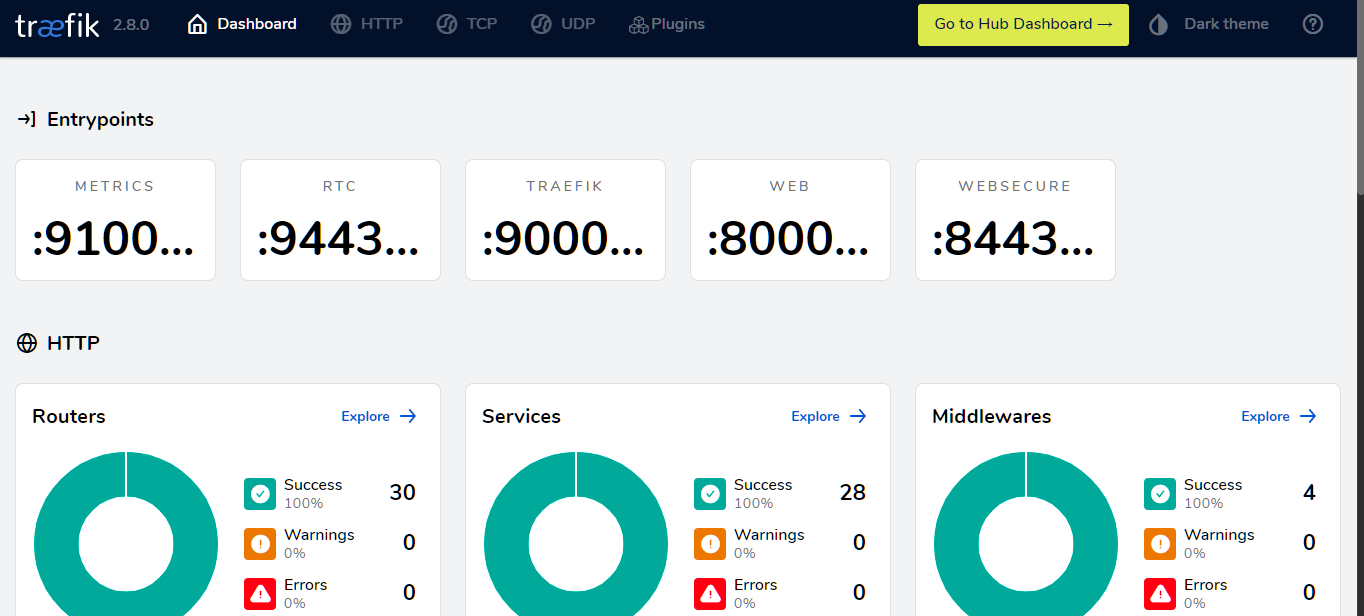
\includegraphics[width=1.0\textwidth,angle=00]{assets/f25.png}
\caption{ Dashboard of traefik }
\label{fig:dashboard of traefik}
\end{figure}

Notice that traefik has multiple entrypoints configured depending on the protocol and the use case. The main entrypoint is websecure. It regulates the HTTPS traffic.  

When Traefik receives an incoming request, it can use the TLS Store to look up the appropriate certificate for the requested domain and use it to encrypt and decrypt traffic. 

Traefik is used in combination with the security layer services to allow for authenticating and authorizing access. The security layer will be discussed in detail further in this report. 

\subsection{Layer 4 load balancing: network level }

In this level, load balancing is mostly related to the network, IP addresses, network address translation ( NAT ), and packets. 

\begin{enumerate}[label = (\alph*)]

\item Using the built in Kubernetes capability : NodePort services 
The NodePort Service exposes a deployment or a set of pods by mapping a specific port on each node in the cluster to the port of the service. 
This allows external clients to access the service by connecting to any of the nodes in the cluster. 
Here's how NodePort Services work: 
    \begin{enumerate}[label = (\arabic*)]
    \item A NodePort Service is defined as a Kubernetes object with the           "type: NodePort" field in the YAML manifest. 
    \item When a NodePort Service is created, Kubernetes assigns a high port number (in the range 30000-32767) to the service. 
    \item Kubernetes then maps the assigned port to the port of the service, which can be any valid port number. 
    \item The NodePort Service is then exposed on all nodes in the cluster, allowing external clients to access the service by connecting to any of the nodes on the assigned port. 
    \item Traffic received on the assigned port is forwarded to the service's target port, which is the port on which the service is listening. 
    \item Kubernetes ensures that the traffic is load balanced across all pods that are part of the service. 
    \end{enumerate}

\item Using metalLB for load balancing : LoadBalancer services 
MetalLB is used to provide network load balancing for services running in the cluster. Here's how MetalLB works in our Kubernetes cluster: 

    \begin{itemize}[label={--}]
        \item MetalLB is deployed in the cluster using the following manifests: 
            \begin{enumerate}[label = (\arabic*)]
            \item "metalLB\_configmap.yml": a configmap resource containing the ip address pool that metalLB is allowed to use to allocate to loadbalancer-type services. As a sample, here is the code snippet for this configmap, the rest will be added in the index section of this document : 

            \begin{listing}
            \inputminted{Yaml}{codeListing/metalLB_configmap.yml}
            \caption{Cert manager certificate }
            \label{lst:metalLB}
            \end{listing}

            \item "metalLB\_rbac.yml": a method of providing fine-grained access control in Kubernetes. RBAC is a security mechanism that restricts access to resources and operations based on the roles assigned to users or service accounts in the cluster. 
            \item "metalLB\_service\_account.yml": an identity that is used by a pod or a set of pods to access the Kubernetes API server and other resources in the cluster. 
            \item "metalLB\_controller.yml": a deployment that watches for changes to load balancer services in the cluster and dynamically assigns IP addresses to those services as needed. 
            \item "metalLB\_speaker.yml": a daemonset that spawns a pod in every node in the cluster it is responsible for announcing the allocated IP addresses for load balancer services. 
            \item "metalLB\_pod\_security\_policy.yml": It allows the definition of a set of security policies that pods must comply with to be scheduled and run on nodes in the cluster. In the context of MetalLB, this PSP is used to enforce security measures for the MetalLB components, including the MetalLB controller and the MetalLB speaker. 
            \end{enumerate}

        \item Exposing a workload using the deployed metalLB loadbalancer is as follows: 
            \begin{enumerate}[label = (\arabic*)]
                \item After creating the application deployment, we create a Kubernetes Service that exposes this workload using the "type" field of the Service to "LoadBalancer". 
                \item Once the Service is created, MetalLB will allocate an IP address from the configured pool of addresses and assign it to the Service. 
                \item We then use this IP address to access your workload from outside the cluster. 
            \end{enumerate}
        \item This is a sample service of the "LoadBalancer" type: 
        
        \begin{figure}[H]\centering
        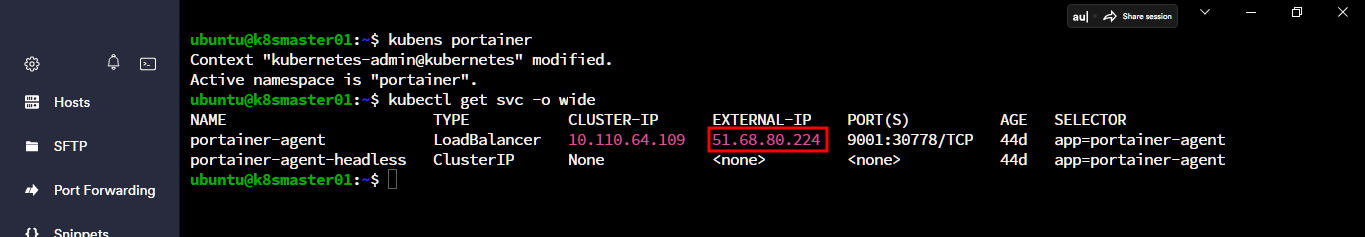
\includegraphics[width=1.0\textwidth,angle=00]{assets/f23.png}
        \caption{LoadBalancer service }
        \label{fig:LoadBalancer}
        \end{figure}
        
    \end{itemize}

\end{enumerate}

\section{Distributed storage backend}

\subsection{Architectural overview on storage}

Distributed persistent storage is important for running stateful applications such as databases that require durable storage. In our context, the ability to store data persistently across multiple nodes in a cluster is implemented using the following architecture: 

\begin{figure}[H]\centering
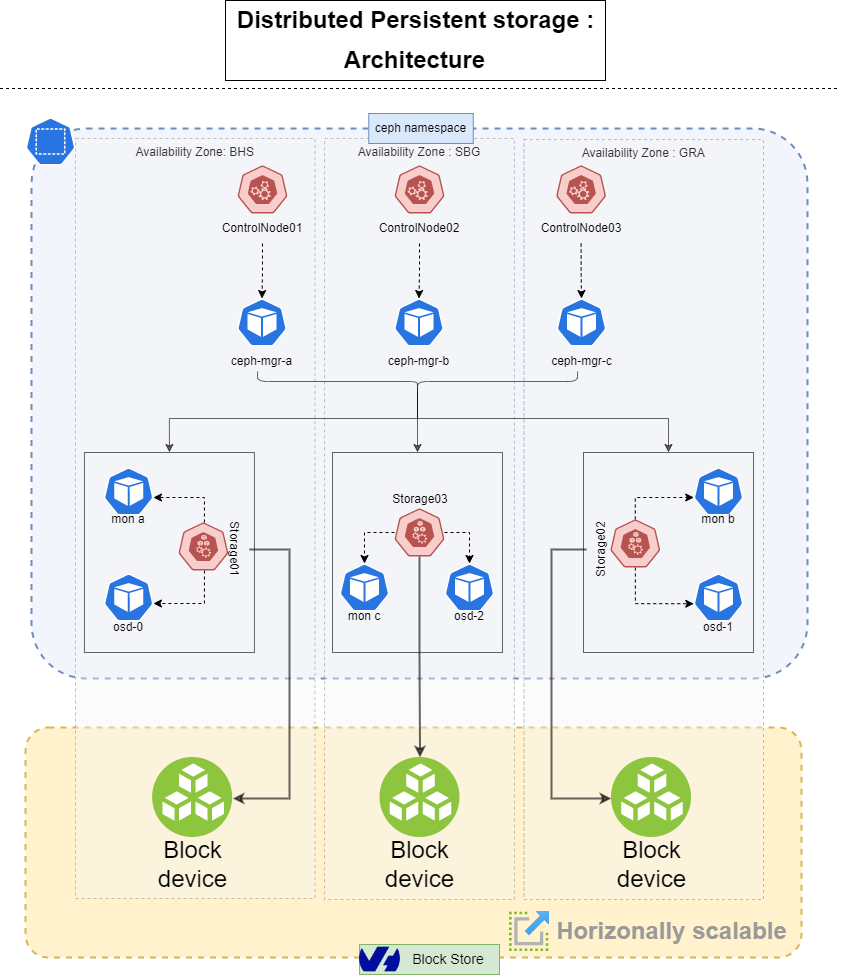
\includegraphics[width=1.0\textwidth,angle=00]{assets/f26.png}
\caption{Architectural overview on storage}
\label{fig:Architectural overview on storage}
\end{figure}

The figure above illustrates a highly scalable storage architecture using “Ceph”. As mentioned in the infrastructure provisioning chapter, in each region, we have created a dedicated storage instance to which a disk the raw format has been attached. The number of disks attached to each node is infinitely scalable and only dependent on the specs of the instance to which it is attached. Furthermore, the size of each disk can be scaled up by the cloud provider. That being said, the number of instances is itself theoretically infinitely scalable. And thus, both horizontal and vertical scalability is achieved. 

\subsection{Ceph as a storage provider for kubernetes }

“Ceph”, our storage provider is deployed as a resource. It includes several components, such as the Ceph monitor, manager, OSD (object storage daemon), and MDS (metadata server), that work together to provide distributed storage: 

\begin{itemize}[label={--}]
    \item First, we deploy the operator, which is a Kubernetes-native controller that automates the deployment and management of the Ceph storage cluster. 
    \begin{figure}[H]\centering
    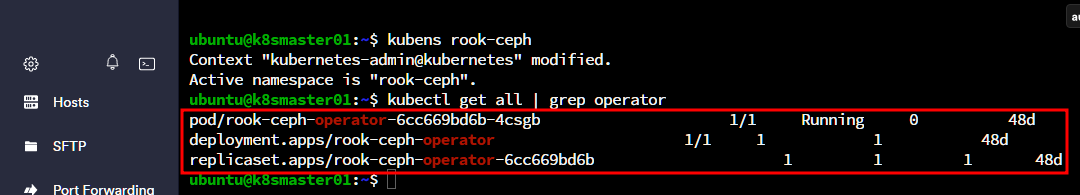
\includegraphics[width=1.0\textwidth,angle=00]{assets/f27.png}
    % \caption{Figure 27 }
    % \label{fig:f27}
    \end{figure}
    \item Next we create a CephCluster custom resource, which defines the desired state of the Ceph cluster.
    \begin{figure}[H]\centering
    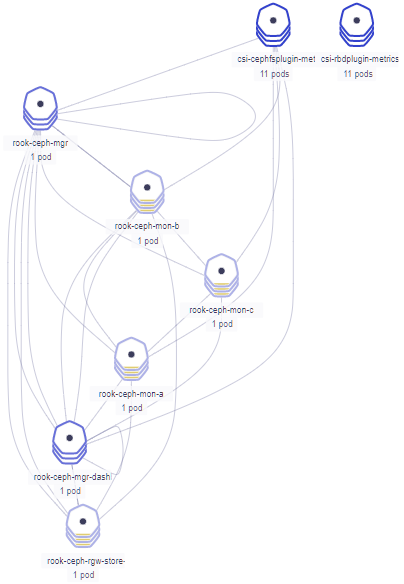
\includegraphics[width=1.0\textwidth,angle=00]{assets/f28.png}
    % \caption{Figure 28 }
    % \label{fig:f28}
    \end{figure}
    \end{itemize}
Ceph is configured such that it will use every raw block device attached to the storage nodes to join it to its storage pool. For each storageNode, the operator spawns an OSD (Object Storage Daemon) which is a storage node that stores objects, e.g., the basic units of data.  
Using the ingress controller, a dashboard for “ceph” is exposed and allows for observability on the storage backend: 
\begin{figure}[H]\centering
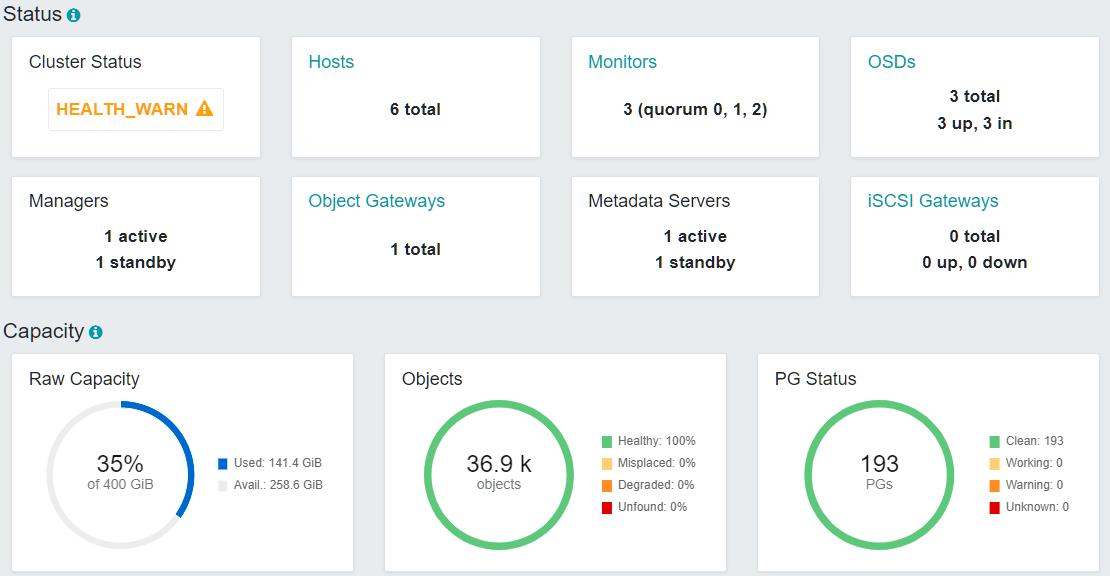
\includegraphics[width=1.0\textwidth,angle=00]{assets/f29.png}
\caption{Ceph Dashboard }
\label{fig:Ceph Dashboard }
\end{figure}

\subsection{Deployed storage capabilities: }

The following diagram provides an overview on the storage capabilities of ceph : 
\begin{figure}[H]\centering
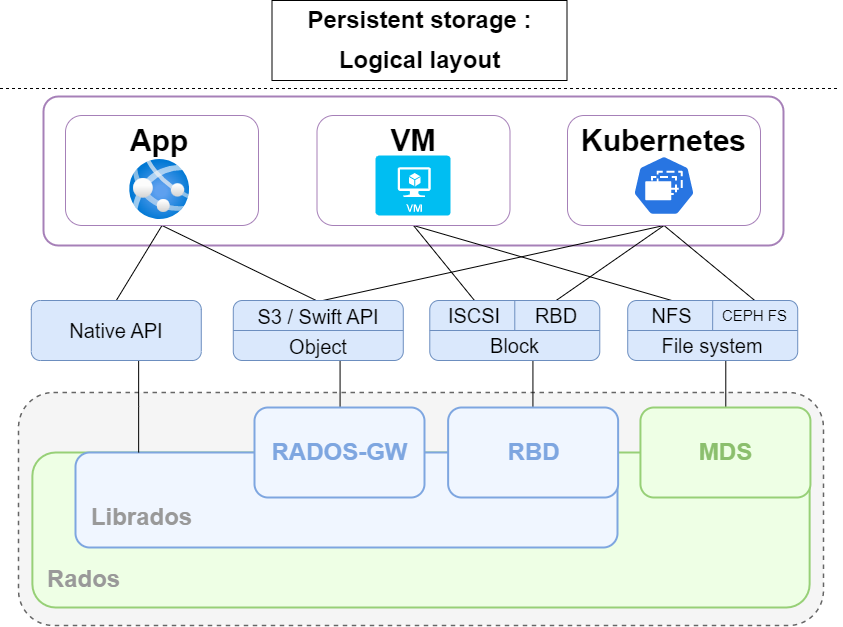
\includegraphics[width=1.0\textwidth,angle=00]{assets/f30.png}
\caption{Storage capabilities Diagram}
\label{fig:f30}
\end{figure}

\subsubsection{Filesystem storage mode: }

CephFS works by creating a virtual file system on top of the RADOS object store, which allows multiple clients to access the same file system concurrently. 

In order to leverage the filesystem storage mode in the service of the deployed workloads in the cluster: 
\begin{enumerate}[label = (\arabic*)]
    \item A CephFilesystem CRD is created. 
    \item Next, a StorageClass that specifies the storage parameters for the file system, such as the size of the file system and the type of file system (e.g., ext4 or xfs). 
    \item A Persistent Volume Claim is created. 
    \item When a pod requests a volume that matches the PVC, Kubernetes (the CSI provisioner) will dynamically provision a volume from the CephFS file system and mount it to the pod. 
\end{enumerate}
As shown by the figure below, CephFS provides built-in redundancy and fault tolerance, ensuring that data is always available even in the event of hardware failures. 
\begin{figure}[H]\centering
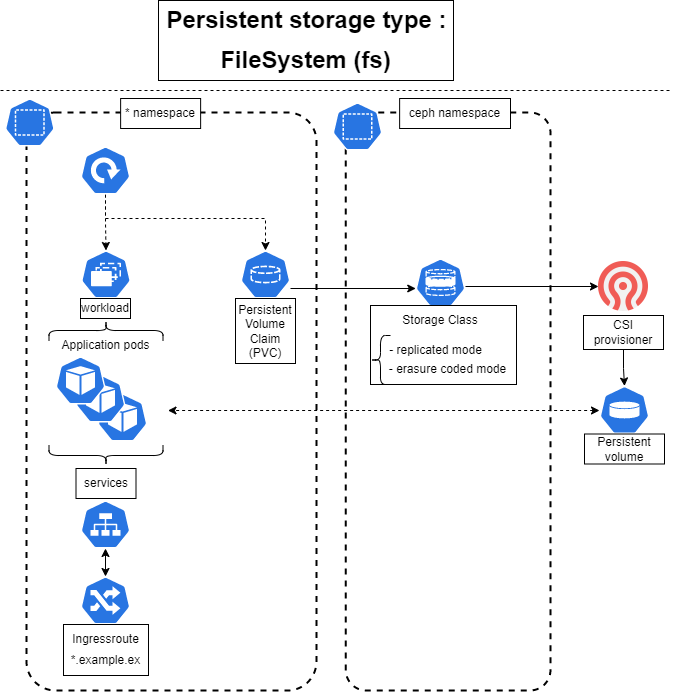
\includegraphics[width=1.0\textwidth,angle=00]{assets/f31.png}
\caption{Filesystem Storage}
\label{fig:Filesystem Storage}
\end{figure}

\subsubsection{Object storage mode: }

It stores data as objects, rather than as files or blocks. This allows applications to store and retrieve large amounts of unstructured data in a highly available and fault-tolerant manner. 

Ceph Object Storage exposes an S3-compatible API. 

The procedure to provision object store buckets is as follows: 

\begin{enumerate}[label = (\arabic*)]
    \item First we create the CephObjectStore CRD that starts the RGW (RadosGateWay) service in the cluster with an S3 API. 
    \item Next, an object store StorageClass is created. It contains such as the reclaimPolicy and the objectStore to which it is linked. 
    \item Finally, for every bucket we desire to create, we either use the S3 API to converse with the RGW or we declare an ObjectBucketClaim which will then be resolved to a bucket. 
\end{enumerate}


This procedure is summarized by the following figure: 

\begin{figure}[H]\centering
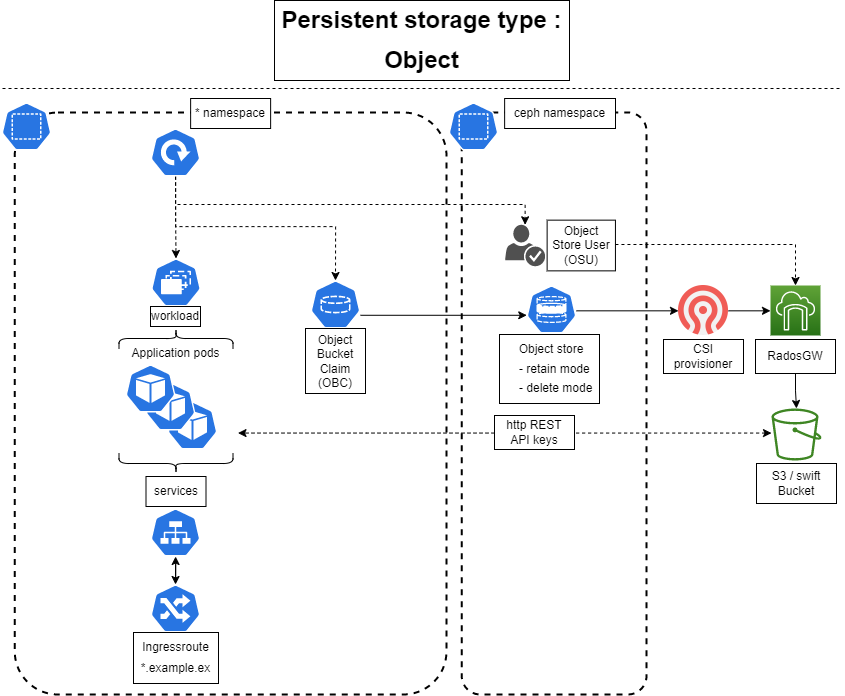
\includegraphics[width=1.0\textwidth,angle=00]{assets/f32.png}
\caption{Object Storage mode }
\label{fig:Object Storage mode}
\end{figure}

\subsubsection{Block storage mode: }

Ceph Block Storage exposes a block device interface. But due to the very nature of a containerized environment, we are not using this capability. The following is a summary on the procedure to provision block devices using ceph: 

\begin{figure}[H]\centering
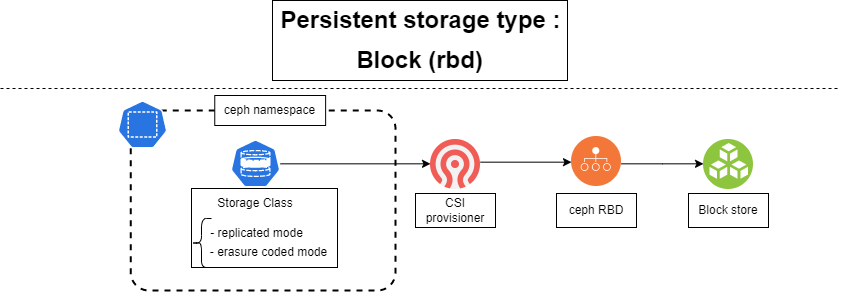
\includegraphics[width=1.0\textwidth,angle=00]{assets/f33.png}
\caption{Block Storage Procedure}
\label{fig:Block Storage Procedure}
\end{figure}

The following are the basic steps involved: 

\begin{enumerate}[label = (\arabic*)]
\item Create the CephBlockPool CRD : defines a specific type of Ceph storage pool. It is used to provision block storage volumes on a Ceph cluster for Kubernetes applications. It specifies a Ceph storage pool with certain parameters, such as the number of replicas, disk size, and disk type. 
\item Create the StorageClass: a Kubernetes StorageClass that references the Ceph cluster. This StorageClass defines the properties of the block storage volumes that will be created, such as the replication factor and the type of storage pool. 
\item Create the PersistentVolumeClaim (PVC): Once the StorageClass is created, we create a PersistentVolumeClaim (PVC) using the StorageClass. This PVC requests a block storage volume of a certain size and other properties defined in the StorageClass. 
\item Attach PVC to Pod: Finally, we attach the PVC to a Kubernetes Pod as a volume. This allows the Pod to use the block storage volume as a local disk. 
\end{enumerate}

When a Pod is created, Kubernetes automatically provisions a block storage volume by creating a block device in the Ceph cluster and attaching it to the Pod. 

When the Pod is deleted, the block storage volume is automatically deleted as well. This is contingent on the parameter “reclaimPolicy: Delete” in the storage class. Otherwise, we define a storage class with the parameter “reclaimPolicy: retain”. 

This provides dynamic and on-demand provisioning of block storage volumes to the applications running on Kubernetes. 

\section*{Conclusion}

This chapter covered the setup of a PaaS environment using Kubernetes, which includes traefik as an ingress controller, cert-manager for TLS provisioning, MetalLB for layer 4 load balancing, and Ceph as a distributed storage backend. 

Traefik enables easy management of ingress routes and load balancing. Cert-manager automates the management of SSL/TLS certificates, making it easy to secure applications. MetalLB provides a simple and straightforward method to load-balance traffic between nodes. 

Finally, Ceph provides distributed storage that is scalable, reliable, and has high performance. 